\documentclass[english,serif,mathserif,xcolor=pdftex,dvipsnames,table]{beamer}
\usetheme[informal]{s3it}
\usepackage{s3it}

\title[Introduction to Python]{%
  A Short and Incomplete Introduction to Python
}
\author[S3IT]{%
  Riccardo Murri \texttt{<riccardo.murri@uzh.ch>}
  \\
  S3IT: Services and Support for Science IT,
  \\
  University of Zurich
}
\date{March~2, 2017}

\begin{document}

% title frame
\maketitle

\begin{frame}
  \begin{center}
    {\Huge Welcome!}
  \end{center}
\end{frame}


\begin{frame}
  \frametitle{What is S3IT?}

  \begin{center}
    {\em ``A partner for data- and \\ compute-intensive science''}

    \+
    \begin{description}
    \item[Enable] researchers and projects to run simulations and data analysis.
    \item[Develop] tools to integrate, automate and scale scientific use cases.
    \item[Provide] access to {\em innovative} infrastructures and technologies.
    \end{description}

    \+
    {\em \small{Want to know more? }\url{http://www.s3it.uzh.ch}}
  \end{center}
\end{frame}


\begin{frame}
  \frametitle{Prerequisites}
  This course assumes a basic experience with computer programming.

  \+
  Any language should do, as long as you are already familiar with
  the concepts of variables and functions.
\end{frame}


\begin{frame}[fragile]
  \frametitle{Python 2 \emph{vs} Python 3}

  There are currently two major versions of Python available, with
  slightly different syntax and features.

  \+
  Python 2.7 is the last release in the 2.x series.

  \+
  Python 3.x has a more polished syntax, removing inconsistencies and
  some historical baggage.

  \+
  But Python 2.x is still the default on most Linux distributions, so
  \textbf{we shall focus on Py2 syntax}.

  \+
  {\footnotesize\em
    Watch a debate between ``Pro'' and ``Contra'' advocates:
    \url{http://www.physik.uzh.ch/~nchiapol/webm/3_1_Python3.webm}}

  \+
  {\footnotesize\em
    Explore the key differences:
    \url{http://tinyurl.com/py2-and-py3-key-differences}}
\end{frame}


\begin{frame}
  \frametitle{Talk outline}
  \begin{enumerate}
  \item Python basics
  \item NumPy and plotting
  \item Pandas and how to query tabular data
  \end{enumerate}
\end{frame}


\begin{frame}
  \frametitle{Next steps}

  The course will be structured as a mixture of slides and hands-on
  sessions for practicing Python programming.

  \+
  So, the very first step is making sure you can access the Jupyter/IPython
  server for running the exercise notebooks.
\end{frame}


\part{Python basics}

\section{How to run Python code}

\begin{frame}[fragile]
  \frametitle{The Python shell, I}
  Python is an \emph{interpreted} language.

  \+
  It also features an interactive
  \href{http://en.wikipedia.org/wiki/REPL}{``shell''} for evaluating
  expressions and statements immediately.

  \+
  The IPython shell is started by invoking the command
  \texttt{ipython} in a terminal window.
\begin{semiverbatim}\tiny
\$ \textbf{ipython}
Python 2.7.13 |Anaconda 4.3.0 (64-bit)| (default, Dec 20 2016, 23:09:15)
Type "copyright", "credits" or "license" for more information.

IPython 5.1.0 -- An enhanced Interactive Python.
?         -> Introduction and overview of IPython's features.
%quickref -> Quick reference.
help      -> Python's own help system.
object?   -> Details about 'object', use 'object??' for extra details.

\textbf{In [1]:}{\color{blue}\normalfont\em \(\leftarrow\) here is where you enter commands}
\end{semiverbatim}
\end{frame}


\begin{frame}
  \frametitle{The IPython notebook, I}

  \begin{columns}[t]
    \begin{column}{0.5\textwidth}
      \begin{center}
        \includegraphics[width=1.00\linewidth]{fig/nb.png}
      \end{center}
    \end{column}
    \begin{column}{0.5\textwidth}
      \small

      A more appealing way of interacting with Python is through the IPython
      notebooks.

      \+
      Notebooks are made of ``cells'', which come in two flavors:
      \begin{itemize}
      \item documentation cells, containing text formatted according to the
        \href{http://commonmark.org/help/}{Markdown} conventions;
      \item code cells, containing arbitrary Python code
      \end{itemize}
    \end{column}
  \end{columns}
\end{frame}


\begin{frame}
  \frametitle{The IPython notebook, II}

  To run Python code in the notebook:
  \begin{itemize}
  \item Type your code in a cell besides the {\ttfamily\bfseries\color{blue}
      In~[~]:} (multiple lines are allowed)
  \item Press \textbf{Ctrl+Enter} to evaluate the cell (prompt changes to
    {\ttfamily\bfseries\color{blue} In~[*]:}) --- or press \textbf{Alt+Enter} to
    evaluate the code \emph{and} open a new code cell.
  \item When the Python kernel has done computing, the result appears \emph{under} the
    code cell marked with a {\ttfamily\bfseries\color{red} Out~[~]:} label.
  \end{itemize}

\end{frame}


\begin{frame}[fragile,fragile]
  \frametitle{The Python shell, II}
  Expressions can be entered at the Python shell prompt (the
  `\texttt{>>>}' at the start of a line); they are evaluated and the
  result is printed:
\begin{semiverbatim}
>>> 2+2
4
\end{semiverbatim}

  \+ Throughout these slides, all Python code marked with `\texttt{>>>}' can
  also be entered and evaluated in the IPython notebook cells:
\begin{semiverbatim}
{\color{blue}\bfseries In [1]:} 2+2
{\color{red}\bfseries Out[1]:} 4
\end{semiverbatim}
\end{frame}


\begin{frame}[fragile]
  \frametitle{Lines of Python code}
  Line of Python code are ended by the ``new line'' character. (I.e., when you
  press the \emph{Enter} key.)

  \+
  A line can be continued onto the next by ending it with the
  character `\texttt{\textbackslash}'; for example:
\begin{semiverbatim}
>>> "hello" + \textbackslash
... " world!"
'hello world!'
\end{semiverbatim}
  The prompt changes to `\texttt{...}' on continuation lines.

  \+\scriptsize
  Reference:
  \url{http://docs.python.org/reference/lexical_analysis.html#line-structure}
\end{frame}


\section{Variables, data types, and operations}

\begin{frame}[fragile]
  \frametitle{String literals, I}
  There are several ways to express string literals in Python.

  \+
  Single and double quotes can be used interchangeably:
\begin{semiverbatim}
>>> "a string" == 'a string'
True
\end{semiverbatim}

  \+
  You can use the single quotes inside double-quoted strings, and viceversa:
\begin{semiverbatim}
>>> a = "Isn't it ok?"
>>> b = '"Yes", he said.'
\end{semiverbatim}
\end{frame}


\begin{frame}[fragile]
  \frametitle{String literals, II}
  Multi-line strings are delimited by three quote characters.
\begin{lstlisting}[showstringspaces=false]
>>> a = """This is a string,
... that extends over more
... than one line.
... """
\end{lstlisting}

  \+ In other words, you need not use the backslashes
  ``\texttt{\textbackslash}'' at the end of the lines.
\end{frame}


\begin{frame}[fragile]
  \frametitle{Operators}
  All the usual unary and binary arithmetic operators are
  defined in Python: \texttt{+}, \texttt{-}, \texttt{*}, \texttt{/},
  \texttt{**}~(exponentiation), \texttt{<<}, \texttt{>>}, etc.

  \+
  Logical operators are expressed using plain English words:
  \texttt{and}, \texttt{or}, \texttt{not}.

  \+
  Numerical and string comparison also follows the usual notation:
  \texttt{<}, \texttt{>}, \texttt{<=}, \texttt{==}, \texttt{!=},
  \ldots

  \+
  \begin{references}
    \tiny
    \begin{itemize}
    \item
      \url{http://docs.python.org/library/stdtypes.html#boolean-operations-and-or-not}
    \item
      \url{http://docs.python.org/library/stdtypes.html#comparisons}
    \end{itemize}
  \end{references}
\end{frame}


\begin{frame}
  \frametitle{Your first exercise}
  %\href{http://www.pythonchallenge.com}{\includegraphics[width=\linewidth]{fig/2to38}}
  \begin{center}
    {\Large How much is \href{http://www.pythonchallenge.com}{$2^{38}$} ?}

    \+
    (You have 1 minute time.)
  \end{center}
\end{frame}


\begin{frame}[fragile]
  \frametitle{Operators, II}
  Some operators are defined for non-numeric types:
\begin{lstlisting}
>>> "U" + 'ZH'
'UZH'
\end{lstlisting}

  \+
  Some support operands of mixed type:
\begin{lstlisting}
>>> "a" * 2
'aa'
>>> 2 * "a"
'aa'
\end{lstlisting}

  \+
  Some do not:
\begin{lstlisting}[basicstyle=\footnotesize\ttfamily]
>>> "aaa" / 3
Traceback (most recent call last):
  File "<stdin>", line 1, in <module>
TypeError: unsupported operand type(s) for /: 'str' and 'int'
\end{lstlisting}
\end{frame}


% \begin{frame}[fragile]
%   \frametitle{Operators, III}
%   The ``\texttt{\%}'' operator computes the remainder of integer division.
%   \begin{lstlisting}
%     >>> 9 % 2
%     1
%   \end{lstlisting}
% \end{frame}


\begin{frame}[fragile]
  \frametitle{String interpolation}
  The \lstinline|.format()| method can be used to substitute values into placeholder
  strings.

  \+
  Placeholders can indicate substitutions by ordinal number:
\begin{lstlisting}[basicstyle=\footnotesize\ttfamily]
>>> "This is slide ~\alt<2>{\HL{\small\ttfamily\{0\}}}{\small\ttfamily\{0\}}~ of ~\alt<2>{\HL{\small\ttfamily\{1\}}}{\small\ttfamily\{1\}}~".format(20, 1001)
'This is slide 20 of 1001.'
\end{lstlisting}

  \+
  You can use names instead of numbers (then the order parameter occur in
  \lstinline|format()| does not matter):
\begin{lstlisting}[basicstyle=\footnotesize\ttfamily]
>>> "Today is ~\alt<3>{\HL{\small\ttfamily\{month\}}}{\{month\}}~ ~\alt<3>{\HL{\small\ttfamily\{day\}}}{\small\ttfamily\{day\}}~".format(day=2, month='March')
'Today is March 2'
\end{lstlisting}

  \begin{references}
    \url{https://pyformat.info/}
  \end{references}
\end{frame}


\begin{frame}[fragile]
  \frametitle{Assignment, I}
  Assignment is done via the `\texttt{=}' statement:
\begin{semiverbatim}
>>> a = 1
>>> print(a)
1
\end{semiverbatim}

  \+
  There are a few shortcut notations:
  \begin{itemize}
  \item[] \texttt{\emph{a} += \emph{b}} short for \texttt{\emph{a} = \emph{a} + \emph{b}},
  \item[] \texttt{\emph{a} -= \emph{b}} short for \texttt{\emph{a} = \emph{a} - \emph{b}},
  \item[] \texttt{\emph{a} *= \emph{b}} short for \texttt{\emph{a} = \emph{a} * \emph{b}},
  \item[]   etc. --- one for every legal operator.
  \end{itemize}
\end{frame}


\begin{frame}[fragile]
  \frametitle{Assignment, II}

  \textbf{Python variables are just ``names'' given to values.}

  \+
  This allows you to \emph{reference} the string \texttt{'Python'}
  by the \emph{name} \texttt{a}.  But also by another name \texttt{b}:

  \+
  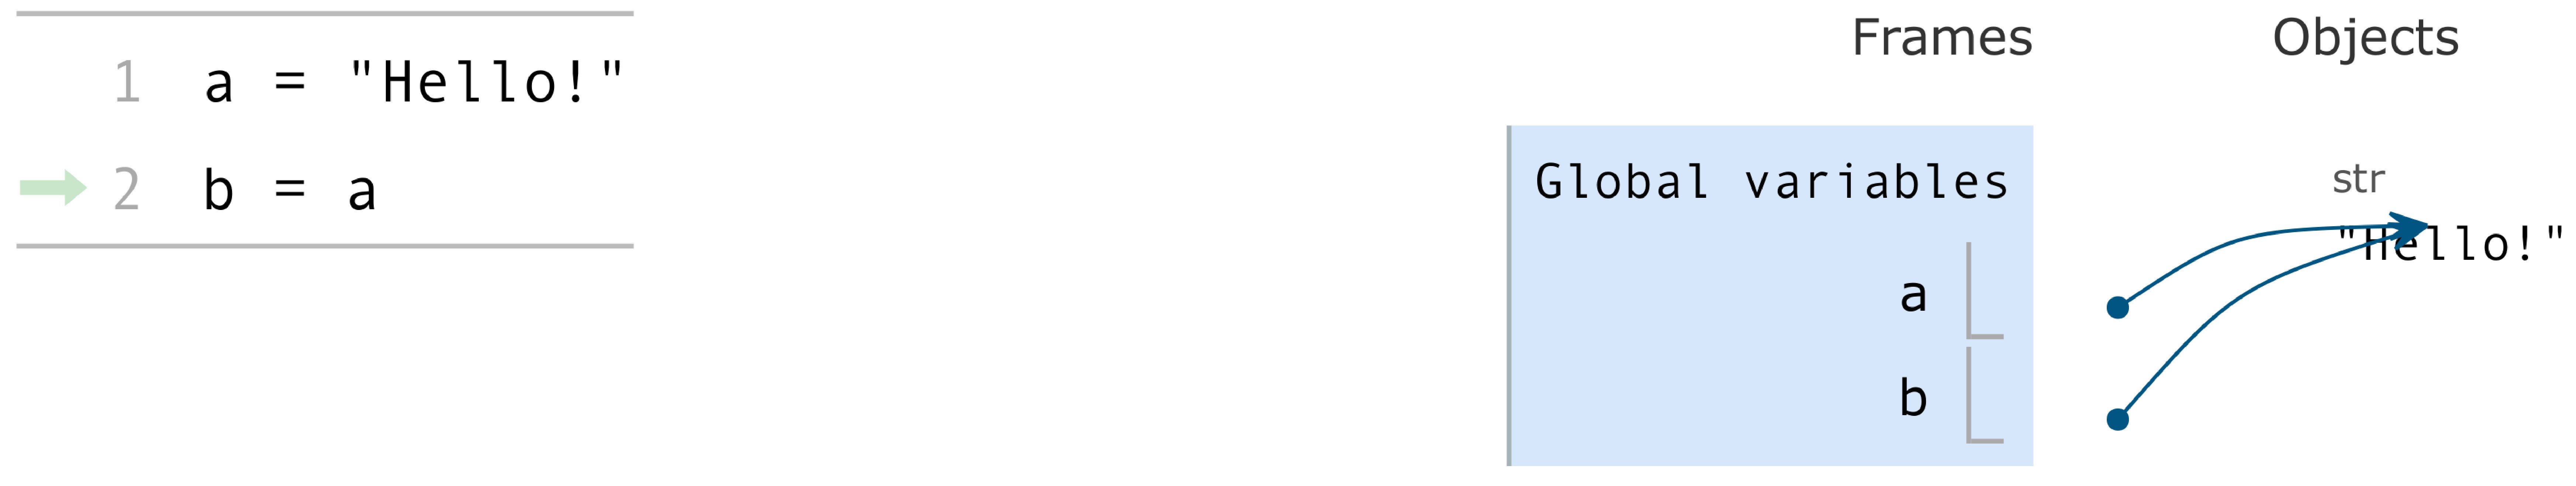
\includegraphics[width=1.00\linewidth]{fig/a=b.pdf}

  \+
  The \emph{same} object can be given many names!

  \+
  \begin{seealso}
    \scriptsize \url{http://excess.org/article/2014/04/bar-foo/}
  \end{seealso}
\end{frame}


\begin{frame}[fragile]
  \frametitle{The \texttt{is} operator}

  The \texttt{is} operator allows you to test whether two names refer
  to the same object:
\begin{lstlisting}
>>> a = 1
>>> b = 1
>>> a is b
True
\end{lstlisting}

\end{frame}


\section{Functions}

\begin{frame}[fragile,label=func1]
  \frametitle{Functions, I}
  Functions are called by postfixing the function name with a
  parenthesized argument list.

  \+
\begin{lstlisting}
>>> int("42")
42
>>> int(4.2)
4
>>> float(42)
42.0
>>> str(42)
'42'
>>> str()
''
\end{lstlisting}
\end{frame}


\begin{frame}[fragile]
  \frametitle{Functions, II}
  Some functions can take a variable number of arguments. For instance:

  \+
  \begin{description}
    \item[sum($x_0$, \ldots, $x_n$)] Return $x_0 + \cdots + x_n$.
    \item[max($x_0$, \ldots, $x_n$)] Return the maximum of $\{ x_0, \ldots, x_n \}$
    \item[min($x_0$, \ldots, $x_n$)] Return the minimum of $\{ x_0, \ldots, x_n \}$
  \end{description}

  \+
  Examples:
\begin{semiverbatim}
>>> min(1,2,3)
1
>>> max(1,2)
2
\end{semiverbatim}
\end{frame}


\begin{frame}[fragile]
  \frametitle{The most important function of all}
  \begin{description}
  \item[help(\texttt{fn})] Display help on the function named \texttt{fn}
  \end{description}

  \+
  \begin{question}
    What happens if you type these at the prompt?
    \begin{itemize}
    \item \texttt{help(abs)}
    \item \texttt{help(help)}
    \end{itemize}
  \end{question}
\end{frame}


\begin{frame}[fragile]
  \frametitle{How to define new functions}
  \begin{columns}[t]
    \begin{column}{0.5\textwidth}
\begin{lstlisting}
~\HL{\textbf{def} greet(name):}~
  """
  A friendly function.
  """
  print ("Hello, " + name + "!")

# the customary greeting
greet("world")
\end{lstlisting}
    \end{column}
    \begin{column}{0.5\textwidth}
      \raggedleft
      The \textbf{def} statement starts a function definition.
    \end{column}
  \end{columns}
\end{frame}

\begin{frame}[fragile]
  \begin{columns}[t]
    \begin{column}{0.5\textwidth}
\begin{lstlisting}
def greet(name):
  """
  A friendly function.
  """
  ~\HL{print ("Hello, " + name + "!")}~

# the customary greeting
greet("world")
\end{lstlisting}
    \end{column}
    \begin{column}{0.5\textwidth}
      \raggedleft
      \textbf{Indentation is significant in Python}: it is used to delimit
      blocks of code, like `\texttt{\{}' and `\texttt{\}}' in Java and C.
    \end{column}
  \end{columns}
\end{frame}

\begin{frame}[fragile]
  \begin{columns}[t]
    \begin{column}{0.5\textwidth}
\begin{lstlisting}
def greet(name):
  """
  A friendly function.
  """
  print ("Hello, " + name + "!")

~\HL{\it\tt\#\ the customary greeting}~
greet("world")
\end{lstlisting}
    \end{column}
    \begin{column}{0.5\textwidth}
      \raggedleft
      (This is a comment. It is ignored by Python, just like blank lines.)
    \end{column}
  \end{columns}
\end{frame}

\begin{frame}[fragile]
  \begin{columns}[t]
    \begin{column}{0.5\textwidth}
\begin{lstlisting}
def greet(name):
  """
  A friendly function.
  """
  print ("Hello, " + name + "!")

# the customary greeting
~\HL{greet("world")}~
\end{lstlisting}
    \end{column}
    \begin{column}{0.5\textwidth}
      \raggedleft
      This calls the function just defined.
    \end{column}
  \end{columns}
\end{frame}

\begin{frame}[fragile]
  \begin{columns}[t]
    \begin{column}{0.5\textwidth}
\begin{lstlisting}
def greet(name):
  ~\HL{"""}~
  ~\HL{A friendly function.}~
  ~\HL{"""}~
  print ("Hello, " + name + "!")

# the customary greeting
greet("world")
\end{lstlisting}
    \end{column}
    \begin{column}{0.5\textwidth}
      \raggedleft
      What is this? The answer in the next exercise!
    \end{column}
  \end{columns}
\end{frame}

\begin{frame}
  \begin{exercise*}[3]
    Type and run the code on the previous page at the interactive
    prompt. (Pay attention to indentation!)

    \+
    What's the result of evaluating the function \texttt{greet("world")}?

    \+
    What does \texttt{help(greet)} output?
  \end{exercise*}
\end{frame}


\begin{frame}[fragile]
  \frametitle{Default values}

  Function arguments can have default values.
\begin{lstlisting}
>>> def hello(name='world'):
...   print ("Hello, " + name)
...
>>> hello()
'Hello, world'
\end{lstlisting}
\end{frame}


\begin{frame}[fragile]
  \frametitle{Named arguments}
Python allows calling a function with named arguments:
\begin{lstlisting}
hello(name="Alice")
\end{lstlisting}

\+
When passing arguments by name, they can be passed in any order:
\begin{lstlisting}
>>> from fractions import Fraction
>>> Fraction(numerator=1, denominator=2)
Fraction(1, 2)
>>> Fraction(denominator=2, numerator=1)
Fraction(1, 2)
\end{lstlisting}
\end{frame}

\begin{frame}[fragile]
  \frametitle{The `return` statement}

  \begin{columns}
    \begin{column}{0.5\textwidth}
      \begin{lstlisting}
def double(x):
  ~\HL{return x+x}~

double(3) == 6
      \end{lstlisting}
    \end{column}
    \begin{column}{0.5\textwidth}
      \raggedleft The result of a function evaluation is set by the
      \textit{return} statement.

     \+
      If no \texttt{return} is present, the function returns the
      special value \texttt{None}.

         \end{column}
  \end{columns}
\+
  \begin{columns}
    \begin{column}{0.5\textwidth}
      \begin{lstlisting}
def double(x):
  return x+x
  # the following line
  # is never exec'd
  ~\HL{print('Hello')}~
      \end{lstlisting}
    \end{column}
    \begin{column}{0.5\textwidth}
      \raggedleft After executing \texttt{return} the control flow
      leaves the function.
    \end{column}
  \end{columns}

\end{frame}

\begin{frame}[fragile]
  \frametitle{Conditionals}
  Conditional execution uses the \texttt{if} statement:
\begin{lstlisting}
if ~\it expr~:
  # indented block
elif ~\it other-expr~:
  # indented block
else:
  # executed if none of the above matched
\end{lstlisting}

  \+The \texttt{elif} can be repeated, with different conditions, or
  left out entirely.

  \+
  Also the \texttt{else} clause is optional.

  \+
  \begin{question}
    Where's the `end if'?

    \pause{There's no `end if': indentation delimits blocks!}
  \end{question}
\end{frame}


\begin{frame}[fragile]
  \frametitle{\texttt{while}-Loops}
  Conditional looping uses the \texttt{while} statement:
\begin{lstlisting}
while ~\it expr~:
  # indented block
\end{lstlisting}
% else:
%   # executed at natural end of the loop

  \+
  To break out of a \texttt{while} loop, use the \texttt{break}
  statement.

  \+
  Use the \texttt{continue} statement anywhere in the indented
  block to jump back to the \texttt{while} statement.

  % \+
  % If a loop is exited via a \texttt{break} statement, the
  % \texttt{else} clause is \emph{not} executed.

  % \+
  % The \texttt{else} clause is optional.
\end{frame}


\begin{frame}
  \begin{exercise*}[4]
    Modify the \texttt{greet()} function to print ``Welcome back!'' if the
    argument \texttt{name} is the string \texttt{'BrainHack'}.
  \end{exercise*}
\end{frame}


\section{Modules}

\begin{frame}[fragile]
  \frametitle{Modules, I}
  The \texttt{import} statement reads a \texttt{.py} file, executes
  it, and makes its contents available to the current program.
\begin{lstlisting}
>>> import hello
Hello, world!
\end{lstlisting}

  \+
  \textbf{Modules are only read once}, no matter how many times an
  \texttt{import} statement is issued.
\begin{lstlisting}
>>> import hello
Hello, world!
>>> import hello
>>> import hello
\end{lstlisting}

\end{frame}


\begin{frame}[fragile]
  \frametitle{Modules, II}
  Modules are \emph{namespaces:} functions and variables defined in
  a module must be prefixed with the module name when used in other
  modules:
\begin{lstlisting}
>>> hello.greet("Python")
Hello, Python!
\end{lstlisting}

  \+
  To import definitions into the current namespace, use the
  `\texttt{from $x$ import $y$}' form:
\begin{lstlisting}
>>> from hello import greet
>>> greet("Python")
Hello, Python!
\end{lstlisting}
\end{frame}


\section{Lists and \texttt{for}-loops}

\begin{frame}
  \frametitle{Sequences}

  Python provides a few built-in \emph{sequence} classes:
  \begin{description}
  \item[list] \emph{mutable}, possibly heterogeneous
  \item[tuple] \emph{immutable}, possibly heterogeneous
  \item[str] \emph{immutable}, only holds characters
  \end{description}

  \+
  Additional sequence types are provided by external modules:
  \begin{description}
  \item[array] \emph{mutable}, homogeneous (like C/Fortran arrays,
    from~\href{http://numpy.scipy.org}{NumPy})
  \item[DataFrame] \emph{mutable}, heterogeneous (like R,
    from~\href{http://pandas.pydata.org/}{Pandas})
  \end{description}

\end{frame}


\begin{frame}[fragile]
  \frametitle{Lists - \textit{(mutable, heterogeneous)}}
  Lists are by far the most common and used sequence type in Python.

  \+
  Lists are created and initialized by enclosing values into
  `\texttt{[}' and `\texttt{]}':
\begin{lstlisting}
>>> L = [ 'U', 'Z' ]
\end{lstlisting}

  \+\pause
  You can append and remove items from a list:
\begin{lstlisting}
>>> L.append('H')
>>> print (L)
['U', 'Z', 'H']
\end{lstlisting}

  \+\pause
  You can append \textbf{any} object to a list:
\begin{lstlisting}
>>> L.append([1, 2])
>>> print(L)
['U', 'Z', 'H', [1, 2]]
\end{lstlisting}

  % % \+
  % \begin{references}
  %   \url{http://docs.python.org/tutorial/datastructures.html#more-on-lists}
  % \end{references}
\end{frame}


\begin{frame}[fragile,fragile]
  \frametitle{Sequences, II}
  You can access individual items in a sequence using the postfix
  \texttt{[]} operator.

  \+
  Sequence indices start at 0.

\begin{lstlisting}
>>> L = ['U', 'Z', 'H']
>>> print(L[0], L[1], L[2])
'U' 'Z' 'H'
>>> S = 'UZH'
>>> print(S[0], S[1], S[2])
'U' 'Z' 'H'
\end{lstlisting}
\end{frame}


\begin{frame}[fragile]
  \frametitle{Sequence length}
The \texttt{len()} function returns the number of items in any
  sequence (not just lists).
\begin{lstlisting}
>>> len(L)
3
\end{lstlisting}

  \+ Built-in functions \lstinline|sum()|, \lstinline|max()|, \lstinline|min()|
  also work on list arguments.
\end{frame}


\begin{frame}
  \begin{exercise*}[6]
    Write a function \texttt{avg()} that takes a list of numbers and returns
    their mean value.
  \end{exercise*}
\end{frame}


\begin{frame}[fragile]
  \frametitle{Slices}
  The notation \texttt{[$n$:$m$]} is used for accessing a \emph{slice}
  of sequence (the items at positions $n$, $n+1$, \ldots, $m-1$).

\begin{lstlisting}
>>> # list numbers from 0 to 9
>>> R = list(range(0,10))
>>> R[1:4]
[1, 2, 3]
\end{lstlisting}

  \+
  If $n$ is omitted it defaults to 0, if $m$ is omitted it defaults to
  the length of the sequence.

  \+ A \textit{slice} of a sequence is a sequence \textit{of the same
  type}.
\begin{lstlisting}
>>> S = 'zurich'
>>> S[0:4]
'zuri'
\end{lstlisting}
\end{frame}


\begin{frame}[fragile]
  \frametitle{List mutation}
  You can replace items in a \emph{mutable} sequence by assigning them
  a new value:
\begin{lstlisting}
>>> L = ['U', 'Z', 'H']
>>> L[2] = 'G'
>>> print(L)
['U', 'Z', 'G']
\end{lstlisting}

% \pause
% You can also replace an entire slice of a mutable sequence:
% \begin{lstlisting}
% >>> L[1:3] = ['a', 'b']
% >>> print(L)
% ['U', 'a', 'b']
% \end{lstlisting}

% \pause
% The new slice does not need to have the same length:
% \begin{lstlisting}
% >>> L[2:] = range(5)
% >>> print(L)
% ['U', 'a', 0, 1, 2, 3, 4]
% \end{lstlisting}
\end{frame}


\begin{frame}[fragile]
  \frametitle{Operating on lists}

  Python provides a number of methods to modify a list:

  \begin{describe}{L.append(x)}
    Append item \texttt{x} to list \texttt{L}.
  \end{describe}

  \begin{describe}{L.insert(n, x)}
    Insert item \texttt{x} at position \texttt{n} of list \texttt{L};
    other items are ``shited to the right'' to make place.
  \end{describe}

  \begin{describe}{L.remove(x)}
    Remove first occurence of item having value \texttt{x} from list \texttt{L}.
  \end{describe}

  \begin{describe}{L.pop(n)}
    Remove item at position \texttt{n} from list \texttt{L}.
  \end{describe}
\end{frame}


\begin{frame}[fragile]
  \frametitle{Operating on lists, II}

  \begin{describe}{L.index(x)}
    Return position of first item in \texttt{L} having value \texttt{x}.
  \end{describe}

  \begin{describe}{L.count(x)}
    Return number of items in \texttt{L} having value \texttt{x}.
  \end{describe}

  \begin{describe}{L.extend(K)}
    Graft a list \texttt{K} to the end of list \texttt{L}.
  \end{describe}

  \begin{references}
    \url{https://docs.python.org/2/library/stdtypes.html#typesseq}
  \end{references}
\end{frame}


\begin{frame}[fragile]
  \frametitle{Lists operators}
  You can concatenate two lists using the \texttt{+} operator:
  \begin{lstlisting}
>>> [1, 2] + [3, 4]
[1, 2, 3, 4]
  \end{lstlisting}

  \+
  You can mutate a list in place with the \texttt{+=} operator:
  \begin{lstlisting}
>>> L = [1, 2]
>>> L += [3, 4]
>>> print(L)
[1, 2, 3, 4]
  \end{lstlisting}

\+
The \texttt{*} operator also works on lists:
  \begin{lstlisting}
>>> L = [1, 2]
>>> print(L*3)
[1, 2, 1, 2, 1, 2 ]
  \end{lstlisting}
\end{frame}

%%% for loops

\begin{frame}[fragile]
  \frametitle{\texttt{for}-loops}
    With the  \texttt{for} statement, you can \textbf{loop over the items of
    a sequence}:
\begin{lstlisting}
for i in range(0, 4):
  # loop block
  print (i*i)
\end{lstlisting}

  \+
  To break out of a \texttt{for} loop, use the \texttt{break}
  statement.

  \+
  To jump to the next iteration of a \texttt{for} loop, use the
  \texttt{continue} statement.
\end{frame}


\begin{frame}[fragile]
  The \texttt{for} statement can be used to loop over elements in \emph{any sequence}.

  \+
  \begin{columns}[c]
    \begin{column}{0.5\textwidth}
\begin{lstlisting}
>>> for val in ~\HL{[1,2,3]}~:
...   print(val)
1
2
3
\end{lstlisting}
    \end{column}
    \begin{column}{0.4\textwidth}
      \raggedleft
      Loop over lists
    \end{column}
  \end{columns}
\end{frame}


\begin{frame}[fragile]
  The \texttt{for} statement can be used to loop over elements in \emph{any sequence}.

  \+
  \begin{columns}[c]
    \begin{column}{0.5\textwidth}
\begin{lstlisting}
>>> for val in ~\HL{'UZH'}~:
...   print(val)
'U'
'Z'
'H'
\end{lstlisting}
    \end{column}
    \begin{column}{0.4\textwidth}
      \raggedleft
      Loop over strings
    \end{column}
  \end{columns}
\end{frame}

\begin{frame}[fragile]

  If you want to loop over a \textit{sorted} sequence you can use the
  function \texttt{sorted()} :

  \begin{lstlisting}
>>> for val in sorted([1,3,2]):
...  print(val)
1
2
3
  \end{lstlisting}

and to loop over a sequence in \textit{inverted} order you can use the
\texttt{reversed()} function:

\begin{lstlisting}
>>> for val in reversed('UZH):
...     print(val)
'H'
'Z'
'U'
\end{lstlisting}

\end{frame}


\begin{frame}[fragile]
  \begin{exercise*}[7]
    Write a function \texttt{odd} that takes a list of integers and
    returns a list of all the odd ones.
  \end{exercise*}

  \+
  \begin{exercise*}[8]
    Write a function \texttt{deviation(L, m)} that takes a list \texttt{L} of
    numbers and a single value \texttt{m} returns a list with the difference of
    \texttt{m} and each element \texttt{x} of \texttt{L}.
  \end{exercise*}
\end{frame}


\begin{frame}
  \frametitle{map, reduce, filter (1)}

  Constructing a new list by looping over a given list and applying a function
  on all elements is so common that there are specialized functions for that:

  \begin{describe}{map(fn, L)}
    Return a new list formed by applying function \texttt{fn(x)} to every
    element \texttt{x} of list \texttt{L}
  \end{describe}

  \+
  \begin{describe}{filter(fn, L)}
    Return a new list formed by elements \texttt{x} of list \texttt{L} for which
    \texttt{fn(x)} evaluates to a ``True'' value.
  \end{describe}
\end{frame}

\begin{frame}
  \frametitle{map, reduce, filter (2)}

  \begin{describe}{reduce(fn2, L)}
    Apply function \texttt{fn2(x,y)} to the first two items \texttt{x} and
    \texttt{y} of list \texttt{L}, then apply \texttt{fn2} to the result and the
    third element of \texttt{L}, and so on until all elements have been
    processed --- return the final result.
  \end{describe}

  \+
  \begin{seealso}
    \url{http://www.python-course.eu/lambda.php}
    and \url{https://docs.python.org/3/howto/functional.html} (more advanced)
  \end{seealso}
\end{frame}


\begin{frame}[fragile]
  This is how you could rewrite Exercises~7 and~8 using \texttt{map} and
  \texttt{filter}.

  \begin{columns}
    \begin{column}{0.5\linewidth}
\begin{python}
# *** Exercise 7 ***
def is_odd(x):
  return (x % 2 == 0)

def odd(L):
  return filter(is_odd, L)
\end{python}
\end{column}
\begin{column}{0.5\linewidth}
\begin{python}
# *** Exercise 8 ***
def deviation(L, m):
  # note: can define
  # func's in func's!
  def delta(x):
    return abs(x-m)
  return map(delta, L)
\end{python}
\end{column}
  \end{columns}
\end{frame}

\section{File I/O}

\begin{frame}[fragile]
  \frametitle{File I/O}

  Code for processing a text file usually looks like this:
\begin{lstlisting}
with open(filename, 'r') as stream:
  # prepare for processing
  for line in stream:
    # process each line
\end{lstlisting}
\end{frame}


\begin{frame}[fragile]
  \frametitle{File I/O}

\begin{lstlisting}
with ~\HL{open(filename, 'r')}~ as stream:
  # prepare for processing
  for line in stream:
    # process each line
\end{lstlisting}

  \+ The \lstinline|open(path, mode)| function opens the file located at
  \texttt{path} and returns a ``file object'' that can be used for reading
  and/or writing.

  \+ Mode is one of '\texttt{r}', '\texttt{w}' or '\texttt{a}' for reading,
  writing (truncates on open), appending. You can add a `\texttt{+}' character
  to enable read+write (other effects being the same).
\end{frame}


\begin{frame}[fragile]
  \frametitle{File I/O}

\begin{lstlisting}
~\HL{with}~ open(filename, 'r') ~\HL{as}~ stream:
  # prepare for processing
  for line in stream:
    # process each line
\end{lstlisting}

  \+
  This is equivalent to \lstinline|stream = open(...)| but in addition
  \emph{closes} the file when the code in the \texttt{with}-block is done.

  \+
  There are many more uses of the \texttt{with} statement besides automatically
  closing files, check out \url{https://jeffknupp.com/blog/2016/03/07/python-with-context-managers/}
\end{frame}


\begin{frame}[fragile]
  \frametitle{File I/O}

\begin{lstlisting}
with open(filename, 'r') as stream:
  # prepare for processing
  ~\HL{for line in stream}~:
    # process each line
\end{lstlisting}

  \+ A \texttt{for}-loop can be used to process all lines in a file, as if the
  file were a list.
\end{frame}


% \begin{frame}[fragile]
%   \frametitle{File I/O}

% \begin{lstlisting}
% with open(filename, 'r') as stream:
%   # prepare for processing
%   for line in stream:
%     # process each line
% \end{lstlisting}
% \end{frame}


\begin{frame}[fragile]
  \frametitle{More on File I/O}

  The \lstinline|.read()| method can be used to read the \emph{whole} contents
  of a file in one go as a single string:
\begin{lstlisting}
>>> s = stream.read()
\end{lstlisting}

  \+
  Method \lstinline|.readlines()| returns a list of all lines in the file:
\begin{lstlisting}
>>> L = stream.readlines()
\end{lstlisting}

  \begin{references}
    \url{http://docs.python.org/library/stdtypes.html#file-objects}
  \end{references}
\end{frame}


\begin{frame}[fragile,label=typeconv]
  \frametitle{Type conversions}
  \begin{description}
  \item[str($x$)] Converts the argument $x$ to a string; for numbers,
    the base 10 representation is used.
  \item[int($x$)] Converts its argument $x$ (a number or a string) to an integer;
    if $x$ is a a floating-point literal, decimal digits are truncated.
  \item[float($x$)] Converts its argument $x$ (a number or a string) to a
    floating-point number.
  \end{description}
\end{frame}


\begin{frame}[fragile]
%   \begin{exercise}
%     Write a function \lstinline|cat(filename)| that prints the whole contents of a file.

%     \+
%     Test it with the
%     \href{https://raw.github.com/gc3-uzh-ch/python-course/master/welcome.py}{welcome.py}
%     file:
% \begin{lstlisting}
% >>> cat('welcome.py')
% #! /usr/bin/env python

% print ("Welcome to Python!")
% \end{lstlisting}
%   \end{exercise}
%  \+
  \begin{exercise*}[9]
    Write a function \lstinline|load_data(filename)| that reads a file
    containing one integer number per line, and return a list of the
    integer values.

    \+
    Test it with the
    \href{https://raw.github.com/gc3-uzh-ch/python-course/master/values.dat}{values.dat}
    file:
\begin{lstlisting}
>>> load_data('values.dat')
[299850, 299740, 299900, 300070, 299930]
\end{lstlisting}
  \end{exercise*}
\end{frame}

\begin{frame}[fragile]
  \frametitle{Operations on strings, I}
  \begin{describe}{%
      \lstinline|s.capitalize()|,
      \lstinline|s.lower()|,
      \lstinline|s.upper()|}
    Return a \emph{copy} of the string capitalized / turned all lowercase /
    turned all uppercase.
  \end{describe}

  \begin{describe}{\lstinline|s.split(t)|}
    Split \texttt{s} at every occurrence of \texttt{t} and return a list
    of parts.  If \texttt{t} is omitted, split on whitespace.
  \end{describe}

  \begin{describe}{\lstinline|s.startswith(t)|,
      \lstinline|s.endswith(t)|}
    Return \texttt{True} if \texttt{t} is the initial/final substring
    of \texttt{s}.
  \end{describe}

  \begin{references}
    \url{http://docs.python.org/library/stdtypes.html#string-methods}
  \end{references}
\end{frame}


\begin{frame}[fragile]
  \frametitle{Operations on strings, II}
  \begin{describe}{\lstinline|s.replace(old, new)|}
    Return a \emph{copy} of string \texttt{s} with all occurrences of
    substring \texttt{old} replaced by \texttt{new}.
  \end{describe}

  \begin{describe}{%
      \lstinline|s.lstrip()|,
      \lstinline|s.rstrip()|,
      \lstinline|s.strip()|}
    Return a \emph{copy} of the string with the leading (resp.\ trailing,
    resp.\ leading \emph{and} trailing) whitespace removed.
  \end{describe}

  \begin{references}
    \url{http://docs.python.org/library/stdtypes.html#string-methods}
  \end{references}
\end{frame}


\begin{frame}[fragile]
  \frametitle{Filesystem operations, I}
  \small
  These functions are available from the \texttt{os} module.

  \begin{describe}{\lstinline|os.getcwd()|, \lstinline|os.chdir(path)|}
    Return the path to the current working directory /
    Change the current working directory to \texttt{path}.
  \end{describe}

  \begin{describe}{\lstinline|os.listdir(dir)|}
    Return list of entries in directory \texttt{dir} (omitting
    `\texttt{.}' and `\texttt{..}')
  \end{describe}

  % \begin{describe}{\lstinline|os.mkdir(path)|}
  %   Create a directory; fails if the directory already exists.
  %   Assumes that all parent directories exist already.
  % \end{describe}

  \begin{describe}{\lstinline|os.makedirs(path)|}
    Create a directory; no-op if the directory already exists.
    Creates all the intermediate-level directories needed to contain
    the leaf.
  \end{describe}

  \begin{describe}{\lstinline|os.rename(old,new)|}
    Rename a file or directory from \texttt{old} to \texttt{new}.
  \end{describe}

  \begin{references}
    \url{http://docs.python.org/library/os.html}
  \end{references}
\end{frame}


\begin{frame}[fragile]
  \frametitle{Filesystem operations, II}
  These functions are available from the \texttt{os.path} module.

  \begin{describe}{\lstinline|os.path.exists(path)|, \lstinline|os.path.isdir(path)|, \lstinline|os.path.isfile(path)|}
    Return \texttt{True} if \texttt{path} exists / is a directory / is
    a regular file.
  \end{describe}

  \begin{describe}{\lstinline|os.path.basename(path)|,
      \lstinline|os.path.dirname(path)|}
    Return the base name (the part after the last `\texttt{/}'
    character) or the directory name (the part before the last
    \texttt{/} character).
  \end{describe}

  \begin{describe}{\lstinline|os.path.abspath(path)|}
    Make \texttt{path} absolute (i.e., start with a \texttt{/}).
  \end{describe}

  \begin{references}
    \url{http://docs.python.org/library/os.path.html}
  \end{references}
\end{frame}


\section{Dictionaries}

%%% dictionaries

\begin{frame}[fragile]
  \frametitle{Dictionaries}
  The \texttt{dict} type implements a key/value mapping:
\begin{lstlisting}
>>> D = { }
>>> D['a'] = 1
>>> D[2] = 'b'
>>> D
{'a': 1, 2: 'b'}
\end{lstlisting}

\+
  Dictionaries can be created and initialized using the following syntax:
\begin{lstlisting}
>>> D = { 'a':1, 2:'b' }
>>> D['a']
1
\end{lstlisting}
\end{frame}

\begin{frame}[fragile]
  The \texttt{for} statement can be used to loop over keys of a dictionary:
  \+
  \begin{columns}[c]
    \begin{column}{0.5\textwidth}
\begin{lstlisting}
>>> D = { 'a':1, 'b':2 }
>>> for val in ~\HL{D.keys()}~:
...   print(val)
'a'
'b'
\end{lstlisting}
    \end{column}
    \begin{column}{0.4\textwidth}
      \raggedleft
      Loop over dictionary~\emph{keys}.

      \emph{The \texttt{.keys()} part can be omitted, as it's the
        default!}
    \end{column}
  \end{columns}
\end{frame}

\begin{frame}[fragile]
  If you want to loop over dictionary \emph{values}, you have to
  explicitly request it.

  \+
  \begin{columns}[c]
    \begin{column}{0.5\textwidth}
\begin{lstlisting}
>>> D = dict(a=1, b=2)
>>> for val in ~\HL{D.values()}~:
...   print(val)
1
2
\end{lstlisting}
    \end{column}
    \begin{column}{0.4\textwidth}
      \raggedleft
      Loop over dictionary~\emph{values}

      \emph{The \texttt{.values()} cannot be omitted!}
    \end{column}
  \end{columns}
\end{frame}


%%% Mutable vs immutable

\begin{frame}[fragile]
  \frametitle{Mutable vs Immutable}
  Some objects (e.g., \texttt{tuple}, \texttt{int}, \texttt{str})
  are \emph{immutable} and cannot be modified.
\begin{lstlisting}
>>> S = 'UZH'
>>> S[2] = 'G'
Traceback (most recent call last):
  File "<stdin>", line 1, in <module>
TypeError: 'str' object does not support item assignment
\end{lstlisting}


  \+
  \texttt{list}, \texttt{dict}, \texttt{set} and user-defined objects
  are \emph{mutable} and can be modified in-place.
\end{frame}

\begin{frame}[fragile]
  \frametitle{Dictionary, sets and mutable objects}

  Not all objects can be used as dictionary \emph{keys} or items in a
  set:
  \begin{itemize}
    \item
      \textit{Immutable} objects \textbf{can be} used as \texttt{dict} keys or set items.
    \item
      \textit{Mutable} objects  \textbf{cannot be} used as \texttt{dict} keys or set items.
    \end{itemize}

    \+
    {\footnotesize
      (Explanation for the technically savvy: a dictionary is
      essentially a \href{http://en.wikipedia.org/wiki/Hash_table}{Hash
        Table}, therefore keys of a dictionary must be \textit{hashable}
      objects.  If objects were allowed to mutate, their hash value
      would change too and we would lose the mapping.)}
\end{frame}


\begin{frame}[fragile]
  \frametitle{The `{\ttfamily\bfseries in}' operator (1)}

  Use the \lstinline|in| operator to test for presence of an item in a
  collection.

  \begin{describe}{\lstinline|x in S|}
    Evaluates to \texttt{True} if \lstinline|x| is equal to a \emph{value}
    contained in the \lstinline|S| sequence (list, tuple, set).
  \end{describe}

  \begin{describe}{\lstinline|x in T|}
    Evaluates to \texttt{True} if \lstinline|x| is a substring of
    string \lstinline|T|.
  \end{describe}

\end{frame}


\begin{frame}[fragile]
  \frametitle{The `{\ttfamily\bfseries in}' operator (2)}

  Use the \lstinline|in| operator to test for presence of an item in a
  collection.

  \begin{describe}{\lstinline|x in D| \\ \lstinline|x in D.keys()|}
    Evaluates to \texttt{True} if \lstinline|x| is equal to a \emph{key}
    in the \lstinline|D| dictionary.
  \end{describe}

  \begin{describe}{\lstinline|x in D.values()|}
    Evaluates to \texttt{True} if \lstinline|x| is equal to a \emph{value}
    in the \lstinline|D| dictionary.
  \end{describe}

\end{frame}


\begin{frame}[fragile]
\begin{exercise*}[11]
    Write a function \lstinline|wordcount(filename)| that reads a text
    file and returns a dictionary, mapping words into occurrences
    (disregarding case) of that word in the text.

    \+ For example, using the
    \href{https://raw.github.com/gc3-uzh-ch/python-course/master/lorem_ipsum.txt}{lorem\_ipsum.txt}
    file:
    \begin{lstlisting}
>>> wordcount('lorem_ipsum.txt')
{'and': 3, 'model': 1, 'more-or-less': 1,
 'letters': 1, ...
    \end{lstlisting}

    \+ For the purposes of this
    exercise, a ``word'' is defined as a sequence of letters and the
    character ``-'', i.e., ``e-mail'' and ``more-or-less'' should both
    be counted as a single word.
  \end{exercise*}
\end{frame}


\section{Exception handling}

\begin{frame}[fragile]
  \frametitle{Exceptions}

  ``Exceptions'' is the name given in Python to error conditions.

  \+
  You can write code that intercepts some error conditions and
  reacts appropriately.

  \+
  \begin{seealso}
    \url{http://docs.python.org/library/exceptions.html}
  \end{seealso}
\end{frame}


\begin{frame}[fragile]
  \frametitle{What does an exception look like?}
\begin{lstlisting}
>>> stream.write('foo')
Traceback (most recent call last):
  File "<stdin>", line 1, in <module>
IOError: File not open for writing
\end{lstlisting}
\end{frame}


\begin{frame}[fragile]
  \frametitle{What does an exception look like?}
\begin{lstlisting}
>>> stream.write('foo')
Traceback (most recent call last):
  File "<stdin>", line 1, in <module>
IOError: ~\HL{File not open for writing}~
\end{lstlisting}

  \+
  This is the exception \emph{message}: it is supposed to be read
  by the (human) user.
\end{frame}


\begin{frame}[fragile]
  \frametitle{What does an exception look like?}
\begin{lstlisting}
>>> stream.write('foo')
Traceback (most recent call last):
  File "<stdin>", line 1, in <module>
~\HL{IOError}~: File not open for writing
\end{lstlisting}

  \+ This is the exception \emph{class name}; it is used for catching
  exceptions (syntax in the next slide).
\end{frame}


\begin{frame}[fragile]
\begin{lstlisting}
try:
  # code that might raise an exception
except SomeException:
  # handle some exception
except AnotherException, ex:
  # the actual Exception instance
  # is available as variable `ex'
finally:
  # performed on exit in any case
\end{lstlisting}

  \+
  The optional \lstinline|finally| clause is executed on exit from the
  \lstinline|try| or \lstinline|except| block in \emph{any} case.

  \begin{references}
    \scriptsize
    \url{http://docs.python.org/reference/compound_stmts.html#try}
\end{references}
\end{frame}


\begin{frame}[fragile]
  \frametitle{Raising exceptions in your code}
  Use the \lstinline|raise| statement with an \texttt{Exception}
  instance:
\begin{lstlisting}
if an_error_occurred:
  raise RuntimeError("Spider sense is tingling.")
\end{lstlisting}
\end{frame}


\begin{frame}
  \begin{exercise*}[1]
    \em (See IPython notebook)
  \end{exercise*}
\end{frame}


\section{Caveats}

\begin{frame}[fragile]
  \frametitle{All variables are references}

  In Python, \textbf{all objects are ever passed by reference}.

  \+
  In particular, \textbf{variables always store a reference to an
    object}, never a copy!

  \+
  Hence, you have to be careful when modifying objects:
\begin{lstlisting}
>>> a = [1,2,3]
>>> b = a
>>> b.remove(2)
>>> print(a)
\end{lstlisting}
  \only<1>{%
\vspace{-1.5em}
\begin{semiverbatim}
\emph{???}
\end{semiverbatim}
    \begin{center}
      \textbf{Q}: How many items are in the \texttt{a} list now?
    \end{center}
  }%
  \only<2>{%
\vspace{-1.5em}
\begin{semiverbatim}
[1, 3]
\end{semiverbatim}

   \+
   \href{http://tinyurl.com/cq3tcab}{Run this example} in the
   \href{http://pythontutor.com/}{Online Python Tutor} to better
   understand what's going on.

   \+
   {\small \em
     This applies particularly for variables that capture the arguments
     to a function call!}
}%
\end{frame}


\begin{frame}[fragile]
  \frametitle{All variables are references (demo)}

  \href{http://www.pythontutor.com/}{www.pythontutor.com}
  \+

  \only<1>{\includegraphics[width=1.2\textheight]{fig/t1_screenshot_1.png}}
  \only<2>{\includegraphics[width=1.2\textheight]{fig/t1_screenshot_2.png}}
  \only<3>{\includegraphics[width=1.2\textheight]{fig/t1_screenshot_3.png}}
  \only<4>{\includegraphics[width=1.2\textheight]{fig/t1_screenshot_4.png}}

\end{frame}


\part{NumPy and plotting}

\begin{frame}

  {\Huge See IPython notebook:
    \texttt{02-numpy-and-plotting}}
\end{frame}


\part{Pandas: tabular data manipulation}

\begin{frame}

  {\Huge See IPython notebook:
    \texttt{03-pandas.ipynb}}
\end{frame}


% \begin{frame}
%   \begin{quote}
%     ``Reverend fathers, my letters were not wont either to be so prolix, or to
%     follow so closely on one another. Want of time must plead my excuse for both
%     of these faults. The present letter is a very long one, simply because I had
%     no leisure to make it shorter.''
%   \end{quote}

%   \+
%   {\small\em
%     Blaise Pascal, The Provincial Letters,
%     \href{https://ebooks.adelaide.edu.au/p/pascal/blaise/p27pr/part17.html}{Letter XVI}}
% \end{frame}


\part{Appendix}

\begin{frame}[fragile]
  \frametitle{Basic types}
  Basic object types in Python:
  \begin{description}
  \item[bool] The class of the two boolean constants \texttt{True}, \texttt{False}.
  \item[int] Integer numbers: \texttt{1}, \texttt{-2}, \ldots
  %   up to \texttt{9223372036854775807} (on a 64-bit machine)
  % \item[long] Integer numbers of arbitrary size; Python switches
  %   automatically from \texttt{int} to \texttt{long} when needed.
  \item[float] Double precision floating-point numbers, e.g.:
    \texttt{3.1415}, \texttt{-1e-3}.
  \item[str] Text (strings of byte-size characters).
  %\item[unicode] Strings of UNICODE characters.
  \item[list] Mutable list of Python objects
  \item[dict] Key/value mapping
  \end{description}

  \+ The type of a Python object can be gotten via the \texttt{type()} function:
\begin{semiverbatim}
{\color{blue}\bfseries In [3]:} type('hello')
{\color{red}\bfseries Out[3]:} str
\end{semiverbatim}
\end{frame}


\subsection{Collections}

\begin{frame}
  \frametitle{Other containers}

  The following builtin containers are always available:
  \begin{description}
  \item[dict] \textit{mutable} key/value mapping.
  \item[set] \textit{mutable}, unordered set of \textit{unique} elements.
  \item[frozenset] \textit{immutable}, unordered set of
    \textit{unique} elements.
  \end{description}

  \pause
  Other specialized containers are available in the
  \texttt{collections} module:

  \begin{description}
  \item[dequeue] a generalization of stacks and queues
  \item[namedtuple] similar to a tuple, but allows you to access the
    elements \textit{by name}
  \item[OrderedDict] dictionary that remembers the order that the
    items were inserted.
  \end{description}
\end{frame}

%%% set container

\begin{frame}[fragile]
  \frametitle{Sets (1)} The \texttt{set} type implements an
  \textbf{unordered} container that holds exactly one object per
  equivalence class:
\begin{lstlisting}
>>> S = set()
>>> S.add(1)
>>> S.add('two')
>>> S.add(1)
>>> S
set([1, 'two'])
\end{lstlisting}

\end{frame}


\begin{frame}[fragile]
  \frametitle{Sets (2)}
You can create a set and add elements to it in one go:
\begin{lstlisting}
>>> S2 = set([1, 2, 3, 4])
\end{lstlisting}

and remove elements:

\begin{lstlisting}
>>> S2.remove(2)
>>> S2.pop()
1
>>> S2
set([3,4])
\end{lstlisting}
\end{frame}


\begin{frame}[fragile]
  \frametitle{Sets (3)}
  Sets are often used to get unique values from a list:
  \begin{lstlisting}
>>> L = [1, 1, 2, 2, 3, 3]
>>> set(L)
set([1, 2, 3])
 \end{lstlisting}

\+\pause
Of course, you can also create a list from a set:
\begin{lstlisting}
>>> S = set((1,2,3))
>>> list(S)
[1, 2, 3]
\end{lstlisting}

\+\pause
\begin{question}
  In what order will the set items appear \\ in the resulting list?
\end{question}

\end{frame}

%%% tuples

\begin{frame}[fragile]
  \frametitle{Tuples}
  Tuples are like lists
  \begin{lstlisting}
>>> T = (1, 2, 3)
>>> T[0]
1
>>> T[0:1]
(1,)
  \end{lstlisting}

  \+
but they are \textit{immutable}

\begin{lstlisting}[basicstyle=\footnotesize\ttfamily]
>>> T[0] = 'a'
Traceback (most recent call last):
  File "<stdin>", line 1, in <module>
TypeError: 'tuple' object does not support item assignment
\end{lstlisting}
\end{frame}

% %%% multiple assignment

\begin{frame}[fragile]
\frametitle{Multiple assignment}
% aka "destructuring bind"
You can assing multiple variables at the same time
\begin{lstlisting}
>>> a, b, c = (1, 2, 3)
>>> print(a)
1
>>> print(b)
2
\end{lstlisting}

\+

It works with any sequence:

\begin{lstlisting}
>>> a, b, c = 'UZH'
>>> print(a)
U
\end{lstlisting}

\pause
\begin{question}
  Can you think of a way to swap the values of two variables using this?
\pause
\begin{lstlisting}
>>> a, b = b, a
\end{lstlisting}
\end{question}
\end{frame}

\begin{frame}[fragile]
\frametitle{Multiple assignment (2)}
Multiple assignment can be used in \texttt{for} statements as well.
\begin{lstlisting}
>>> L = [(1,'a'), (2,'b'), (3, 'c')]
>>> for x, y in L:
...     print ("first is " + str(x)
...            + ' and second is ' + y)
\end{lstlisting}

  \+
  This is particularly useful with functions that return a tuple.
  For instance the \texttt{enumerate()} function (look it up with
  \texttt{help()}!).
\end{frame}


%%% data structures recap

\begin{frame}
  \frametitle{Data structures recap}
  \begin{center}
    \begin{tabular}{>{\ttfamily}c|>{\ttfamily}c|>{\footnotesize}p{0.5\linewidth}}
      \rmfamily \textbf{mutable} & \rmfamily \textbf{immutable} & \\
      set & frozenset & unordered container of
      unique elements\\[1ex]
      list & tuple & ordered sequence\\[1ex]
      dict & $-$ & key/values mapping\\[1ex]
      $-$& str & ordered sequence of characters\\
    \end{tabular}
  \end{center}
\end{frame}


% \begin{frame}[fragile]
%   \frametitle{Useful data structures operations}

%   Read {\url{http://docs.python.org/tutorial/datastructures.html}}.

%   \+
%   Really, you will need it.

%   \+
%   And remember that \texttt{dir()} and \texttt{help()} are your friends!
% \end{frame}


\subsection{Making copies}

\begin{frame}[fragile]
  \frametitle{How to copy an object?}
  \begin{lstlisting}
>>> import copy
>>> a = [1, 2]
>>> b = copy.copy(a)
>>> b.remove(1)
>>> print(b)
[2]
>>> print(a)
[1, 2]
  \end{lstlisting}
\end{frame}


\begin{frame}[fragile]
  \frametitle{How to copy an object? (2)}
Note that \texttt{copy.copy} makes a \emph{shallow} copy:
  \begin{lstlisting}
>>> D = { 'a':[1,2], 'b':3 }
>>> print(D['a'])
[1, 2]
>>> E = copy.copy(D)
>>> print(E)
{ 'a':[1, 2], 'b':3 }
>>> E['a'].remove(1)
>>> print(D['a'])
[2]
  \end{lstlisting}
\end{frame}


\begin{frame}[fragile]
  \frametitle{How to copy an object? (3)}
To make a copy of nested data structures, you need \texttt{copy.deepcopy}:
  \begin{lstlisting}
>>> D = { 'a':[1,2], 'b':3 }
>>> print(D['a'])
[1, 2]
>>> E = copy.deepcopy(D)
>>> print(E)
{ 'a':[1, 2], 'b':3 }
>>> E['a'].remove(1)
>>> print(D['a'])
[1, 2]
>>> print(E['a'])
[2]
  \end{lstlisting}
\end{frame}


\subsection{Objects}

\begin{frame}
  \frametitle{What's an \emph{object}?}
  \textbf{A Python object is a bundle of variables and functions.}

  \+
  What variable names and functions comprise an object is defined
  by the object's \emph{class}.

  \+
  From one class specification, many objects can be
  \emph{instanciated}.  Different instances can assign different
  values to the object variables.

  \+
  Variables and functions in an instance are collectively called
  \emph{instance attributes}; functions are also termed \emph{instance
    methods}.
\end{frame}


\begin{frame}[fragile]
  \frametitle{Example: the \texttt{datetime} object, I}
  \begin{columns}[c]
    \begin{column}{0.5\textwidth}
\begin{lstlisting}
>>> from datetime import date
>>> ~\HL{dt1 = date(2012, 9, 28)}~
>>> dt2 = date(2012, 10, 1)
\end{lstlisting}
    \end{column}
    \begin{column}{0.5\textwidth}
      \raggedleft
      To instanciate an object, call the class name like a
      function.
    \end{column}
  \end{columns}
\end{frame}


\begin{frame}[fragile]
  \frametitle{Example: the \texttt{datetime} object, II}
\begin{lstlisting}
>>> dir(dt1)
['__add__', '__class__', ~\ldots~, 'ctime', 'day',
'fromordinal', 'fromtimestamp', 'isocalendar',
'isoformat', 'isoweekday', 'max', 'min', 'month',
'replace', 'resolution', 'strftime', 'timetuple',
'today', 'toordinal', 'weekday', 'year']
\end{lstlisting}

  \+
  The \texttt{dir} function can list all objects attributes.

  \+
  Note there is no distinction between instance variables and
  methods!
\end{frame}


\begin{frame}[fragile]
  \frametitle{Example: the \texttt{datetime} object, III}
  \begin{columns}[c]
    \begin{column}{0.5\textwidth}
\begin{lstlisting}
>>> dt1.day
28
>>> dt1.month
9
>>> dt1.year
2012
\end{lstlisting}
    \end{column}
    \begin{column}{0.5\textwidth}
      \raggedleft
      Access to object attributes is done by suffixing the
      instance name with the attribute name, separated by a dot
      ``\texttt{.}''.
    \end{column}
  \end{columns}
\end{frame}


\begin{frame}[fragile]
  \frametitle{Example: the \texttt{datetime} object, IV}
  \begin{columns}[c]
    \begin{column}[b]{0.5\textwidth}
\begin{lstlisting}
>>> dt1 = date(2012, 9, 28)
>>> dt2 = date(2012, 10, 1)

>>> dt1.day
~\HL{28}~
>>> dt2.day
~\HL{1}~
\end{lstlisting}
    \end{column}
    \begin{column}[b]{0.5\textwidth}
      \raggedleft
      The same attribute can have different
      values in different instances!
    \end{column}
  \end{columns}
\end{frame}


\begin{frame}[fragile]
  \frametitle{Instance methods}
\begin{lstlisting}[showstringspaces=false]
>>> dt1.isoformat()
'2012-09-28'
\end{lstlisting}

  \+
  Invoke an instance method just like any other function.
\end{frame}


\begin{frame}[fragile]
  \frametitle{Everything is an object!}

  The \texttt{dir} built-in function is used to list the attributes of an object.

  \begin{python}
>>> dir("hello!")
  \end{python}
\end{frame}


\begin{frame}[fragile]
  \frametitle{Everything is an object!}

  The \texttt{dir} built-in function is used to list the attributes of an object.

  \begin{python}
>>> ~\HL{dir("hello!")}~
['__add__', '__class__', '__contains__',
 '__delattr__', '__doc__', '__eq__',
 ~\ldots~
'strip', 'swapcase', 'title',
'translate', 'upper', 'zfill']
\end{python}

\+\ldots a string is an object!
\end{frame}


\begin{frame}[fragile]
  \frametitle{Everything is an object!}

  \begin{python}
>>> ~\HL{dir([1,2,3])}~
['__add__', '__class__', '__contains__',
~\ldots~
'append', 'count', 'extend',
'index', 'insert', 'pop',
'remove', 'reverse', 'sort']
\end{python}

\+\ldots a \texttt{list} is an object!
\end{frame}


\begin{frame}[fragile]
  \frametitle{Everything is an object!}
  Indeed, you can do:

  \+
  \begin{python}
>>> "hello world!".split()
['hello', 'world!']
\end{python}

\+
\begin{python}
>>> [1,1,2,3,5].count(1)
2
\end{python}
\end{frame}


\begin{frame}[fragile]
  \frametitle{Everything is an object!}

\begin{python}
>>> ~\HL{dir(1)}~
\end{python}

\end{frame}


\begin{frame}[fragile]
  \frametitle{Everything is an object!}

  \begin{python}
>>> ~\HL{dir(1)}~
['__abs__', '__add__', '__and__',
~\ldots~
'conjugate', 'denominator',
'imag', 'numerator', 'real']
\end{python}

\+\ldots an \texttt{int} is an object!

\+
\begin{python}
>>> (1).numerator
2
>>> (1).denominator
1
\end{python}
\end{frame}


\begin{frame}
  \frametitle{Objects \emph{vs} modules}

  Modules are also namespaces of variables and functions.

  \+
  The dot operator `\texttt{.}' is also used to access variables
  and functions from modules.  The \texttt{dir()} function is also
  used to list variables and functions from modules.

  \+
  But each module has \emph{one and only one} instance in a Python
  program.
\end{frame}

\end{document}

%%% Local Variables:
%%% mode: latex
%%% TeX-master: t
%%% End:
